\section{Outer Measure}
Outer measure can be defined on every set.
\begin{definition}[Outer Measure]
    \label{def:outer_measure}
    \

    $E \subseteq \mathbb{R}^n$ is a set,
    $I$ is a closed interval: $I = \{ x = (x_1, x_2, \cdots, x_n) \in \mathbb{R}^n | a_i \leq x_i \leq b_i, i=1, \cdots, n\}$,
    and $v(I)$ is the volume of the interval $I$, 
    \begin{gather*}
        v(I) = \begin{cases}
            \prod_{i=1}^n (b_i - a_i), &\text{ if } a_i \leq b_i ;\\
            0, &\text{ otherwise} .
        \end{cases}
    \end{gather*}
    For set $E$, consider a \textit{countable} collection of open, nounded intervals that cover $E$,
    $S = \{I_i\}_{i=1}^{\infty}$, in the sense that $E \subseteq \bigcup_{i=1}^{\infty} I_i$.
    For each such collection, consider the sum of the volumes of the intervals in the collection. 
    We define
    \begin{gather}
        \sigma(S) = \sum_{i=1}^{\infty} v(I_i)
    \end{gather}
    The outer measure of $E$, denoted by $m^{*}(E)$, is
    \begin{gather}
        m^{*}(E) = \inf \sigma(S)
    \end{gather}
    the infimum is taken over all countable collections of closed intervals $S$.
\end{definition}

\begin{lemma}\label{lem1}
    \

    If $I$ is a closed interval, then $m^{*}(I) = v(I).$
\end{lemma}
\begin{proof}[Proof of Lemma \ref{lem2}]
    \

    By definition, $I$ covers itself, so $m^{*}(I) \leq v(I)$.
    Given any $\epsilon > 0$,
    $\exists S = \{I_i\}_{i=1}^{\infty}$, a closed interval cover,
    such that $\sigma(S) \leq m^{*}(I) + \epsilon$.
    We need to show that $v(I) \leq \sum_{i=1}^{\infty} v(I_i) = \sigma(S).$
    For each $i$, choose a bigger $I_i^*$,
    such that $I \subseteq int(I_i^*)$ and $v(I_i^*) \leq v(I_i)(1 + \epsilon)$.
    Then we have $I \subseteq \bigcup_{i=1}^{\infty} int(I_i^*)$.
    By compactness of $I$, (The Heine-Borel theorem),
    we can find an integer $N$ such that $I \subseteq \bigcup_{i=1}^{N} int(I_i^*)$,
    hence
    \begin{gather*}
        v(I) \leq \sum_{i=1}^{N} v(I_i^*) \leq (1 + \epsilon) \sum_{i=1}^{N} v(I_i) \leq (1 + \epsilon) \sigma(S).
    \end{gather*}
    So $v(I) \leq \sigma(S)$, if we take infimum over all $S$,
    we have $v(I) \leq m^{*}(I)$.
\end{proof}

From Lemma \ref{lem1}, we can see that the outer measure of the boundary of a closed interval is zero, i.e. $ m^* (\partial I) = 0 $.

\begin{lemma}\label{lem2}
    \

    Suppose we have two setws $E_1 \subseteq E_2$, then
    \begin{gather*}
        m^{*}(E_1) \leq m^{*}(E_2).
    \end{gather*}
\end{lemma}

\begin{lemma}\label{lem3}
    \

    Assume we have infinite sets: $E_1, \cdots, E_{\infty}$, $E_k \subseteq \mathbb{R}^n$, $k \in \mathbb{N}$.
    Let $E = \bigcup_{k=1}^{\infty} E_k$,
    then
    \begin{gather*}
        m^{*}(E) \leq \sum_{k=1}^{\infty} m^{*}(E_k).
    \end{gather*}
\end{lemma}

\begin{proof}[Proof of Lemma \ref{lem3}]
    \

    We may assume that $m^{*}(E_k) < \infty$ for all $k$.
    Given any $\epsilon > 0$, for each $k$,
    we can find a countable collection of closed intervals $S_k = \{I_{i}^{(k)}\}_{i=1}^{\infty}$ such that
    $E_k \subseteq S_k$ and that
    \begin{gather*}
        \sum_{i=1}^{\infty} v(I_{i}^{(k)}) \leq m^{*}(E_k) + \frac{\epsilon}{2^k}.
    \end{gather*}
    Then we can take the union over all $k$ to obtain a countable collection of closed intervals $S = \bigcup_{k=1}^{\infty} S_k$ such that
    \begin{gather*}
        E = \sum_{k=1}^{\infty} E_k \subseteq \bigcup_{k=1}^{\infty} S_k = \bigcup_{k=1}^{\infty} \bigcup_{i=1}^{\infty} I_{i}^{(k)}.
    \end{gather*}
    So the outer measure $m^*(E)$ is bounded by the sum of the outer measures of the individual sets:
    \begin{gather*}
        m^{*}(E) \leq \sigma(S) = \sum_{k=1}^{\infty} \sum_{i=1}^{\infty} v(I_{i}^{(k)}) = \sum_{k=1}^{\infty} \left( m^{*}(E_k) + \frac{\epsilon}{2^k} \right) = \sum_{k=1}^{\infty} m^{*}(E_k) + \epsilon.
    \end{gather*}
\end{proof}

\begin{eg}[Singleton]
    \

    Singleton set $E = \{x\}$, where $x \in \mathbb{R}^n$.
    We can cover $E$ with a single closed interval $I = [x, x]$.
    The volume of this interval is $v(I) = 0$.
    Therefore, the outer measure of a singleton set is $m^{*}(E) = 0$.
\end{eg}
\begin{eg}[Countable Set]
    \

    For a countable set $E = \{x_1, x_2, \cdots, x_k, \cdots\}$,
    we can cover it with a finite collection of closed intervals.
    We can take $E = \bigcup_{k=1}^{\infty} {x_k}$.
    So the outer measure is
    \begin{gather*}
        m^{*}(E) \leq \sum_{k=1}^{n} m^{*}(\{x_k\}) = 0.
    \end{gather*}
    As outer measure is non-negative, we have $m^{*}(E) = 0$.
\end{eg}

\subsection{Cantor Set}
\begin{definition}[Cantor Set]\label{def:cantor_set}
    \

    The Cantor set $C$ is defined as follows:
    \begin{enumerate}
        \item Start with the closed interval $[0, 1]$.
        \item Remove the open middle third $(\frac{1}{3}, \frac{2}{3})$.
        \item Repeat this process for each remaining closed interval.
    \end{enumerate}
    The Cantor set is the intersection of all these sets after infinitely many steps.
    \begin{gather*}
        C = \bigcap_{k=1}^{\infty} C_k,
        \quad \text{where } C_k \text{ is the set obtained after } k \text{ iterations.}
    \end{gather*}
    The Cantor set is uncountable, compact, and has Lebesgue measure zero.
    \begin{gather*}
        m^*(C) \leq m^*(C_k) \leq 2^k \cdot \frac{1}{3^k} \to 0.
    \end{gather*}
\end{definition}

For each $k$, the set $C_k$ consists of $2^k$ closed intervals (with $2^k - 1$ open intervals removed),
each of length $\frac{1}{3^k}$.

\subsection{Cantor Function (Devil's Staircase)}
\begin{definition}[Cantor Function]\label{def:cantor_function}
    The Cantor function $f: [0,1] \to [0,1]$ is defined as follows:
    \begin{enumerate}
        \item On the Cantor set $C$, $f$ is defined by the ternary expansion without using digit 1.
        \item On each removed interval $\left(\frac{a}{3^k}, \frac{b}{3^k} \right)$, $f$ is constant.
        \item $f$ is continuous, non-decreasing, and maps $[0,1]$ onto $[0,1]$.
    \end{enumerate}
    For each iteration, we obtain a series of functions: $f_1, f_2, \cdots$, s.t. $f_k: [0, 1] \to [0, 1]$.
    \begin{gather*}
        \vert f_k - f_m \vert \leq \frac{1}{2^k},
    \end{gather*}
    and that $f_k$ is continuously monotone increasing.
    So $f = \lim_{k \to \infty} f_k$ exists and is a continuous function on $[0,1]$, we call it the Cantor function.
    The Cantor function is also known as the "Devil's Staircase" due to its characteristic step-like appearance.
\end{definition}

\begin{figure}[ht!]
\centering
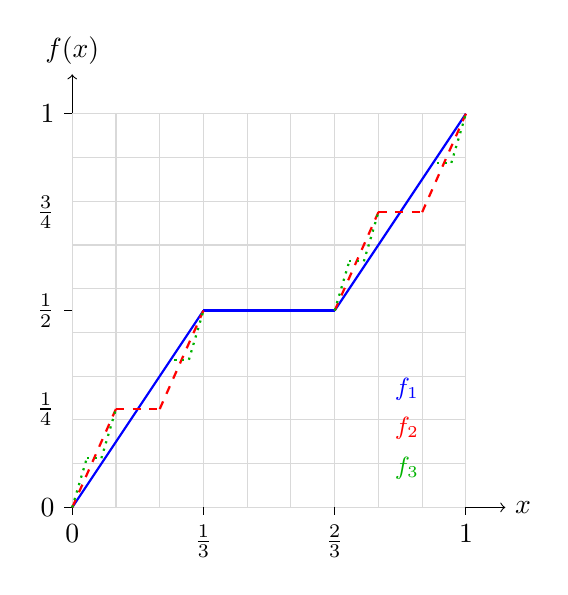
\begin{tikzpicture}[scale=5]
    % Axes
    \draw[->] (0,0) -- (1.1,0) node[right] {$x$};
    \draw[->] (0,0) -- (0,1.1) node[above] {$f(x)$};
    
    % Grid lines
    \draw[gray!30] (0,0) grid[step=1/9] (1,1);
    
    % Tick marks and labels on x-axis
    \foreach \x in {0, 1/3, 2/3, 1} {
        \draw (\x,0) -- (\x,-0.02);
    }
    \node[below] at (0,-0.02) {$0$};
    \node[below] at (1/3,-0.02) {$\frac{1}{3}$};
    \node[below] at (2/3,-0.02) {$\frac{2}{3}$};
    \node[below] at (1,-0.02) {$1$};
    
    % Tick marks and labels on y-axis
    \foreach \y in {0, 1/2, 1} {
        \draw (0,\y) -- (-0.02,\y);
    }
    \node[left] at (-0.02,0) {$0$};
    \node[left] at (-0.02,1/4) {$\frac{1}{4}$};
    \node[left] at (-0.02,1/2) {$\frac{1}{2}$};
    \node[left] at (-0.02,3/4) {$\frac{3}{4}$};
    \node[left] at (-0.02,1) {$1$};
    
    % Cantor function approximation (first few iterations)
    % Level 0: [0,1] -> [0,1]
    % Level 1: constant on (1/3, 2/3)
    \draw[thick, blue] (0,0) -- (1/3,1/2);
    \draw[thick, blue] (1/3,1/2) -- (2/3,1/2);
    \draw[thick, blue] (2/3,1/2) -- (1,1);
    
    % Level 2: constant on (1/9, 2/9) and (7/9, 8/9)
    \draw[thick, red, dashed] (0,0) -- (1/9,1/4);
    \draw[thick, red, dashed] (1/9,1/4) -- (2/9,1/4);
    \draw[thick, red, dashed] (2/9,1/4) -- (1/3,1/2);
    \draw[thick, red, dashed] (2/3,1/2) -- (7/9,3/4);
    \draw[thick, red, dashed] (7/9,3/4) -- (8/9,3/4);
    \draw[thick, red, dashed] (8/9,3/4) -- (1,1);
    
    % Level 3: even finer steps (showing the staircase nature)
    \draw[thick, green!70!black, dotted] (0,0) -- (1/27,1/8);
    \draw[thick, green!70!black, dotted] (1/27,1/8) -- (2/27,1/8);
    \draw[thick, green!70!black, dotted] (2/27,1/8) -- (1/9,1/4);
    \draw[thick, green!70!black, dotted] (7/27,3/8) -- (8/27,3/8);
    \draw[thick, green!70!black, dotted] (8/27,3/8) -- (1/3,1/2);
    
    % Additional fine structure
    \draw[thick, green!70!black, dotted] (2/3,1/2) -- (19/27,5/8);
    \draw[thick, green!70!black, dotted] (19/27,5/8) -- (20/27,5/8);
    \draw[thick, green!70!black, dotted] (20/27,5/8) -- (7/9,3/4);
    \draw[thick, green!70!black, dotted] (25/27,7/8) -- (26/27,7/8);
    \draw[thick, green!70!black, dotted] (26/27,7/8) -- (1,1);
    
    % % Endpoint dots
    % \fill[blue] (0,0) circle (0.8pt);
    % \fill[blue] (1/3,1/2) circle (0.8pt);
    % \fill[blue] (2/3,1/2) circle (0.8pt);
    % \fill[blue] (1,1) circle (0.8pt);
    
    % Legend
    \node[blue] at (0.85,0.3) {\small $f_1$};
    \node[red] at (0.85,0.2) {\small $f_2$};
    \node[green!70!black] at (0.85,0.1) {\small $f_3$};

    % Title
    % \node at (0.5,1.05) {\textbf{Cantor Function (Devil's Staircase)}};
\end{tikzpicture}
% \caption{The Cantor function showing its characteristic "devil's staircase" appearance. The function is constant on each removed interval from the Cantor set construction and increases only on the Cantor set itself.}
\label{fig:cantor_function}
\end{figure}

\begin{remark}
    The Cantor function has several remarkable properties:
    \begin{enumerate}
        \item It is continuous and non-decreasing on $[0,1]$.
        \item It maps $[0,1]$ onto $[0,1]$ surjectively.
        \item Its derivative is zero almost everywhere (on the complement of the Cantor set).
        \item It increases only on the Cantor set, which has measure zero.
        \item It is an example of a singular function: continuous but not absolutely continuous.
    \end{enumerate}
\end{remark}

